\documentclass[tikz,border=8pt]{standalone}
\usepackage{tikz}
\usepackage{tkz-euclide}
\usepackage{amsmath, amssymb}

\usetikzlibrary{angles, quotes}

\begin{document}

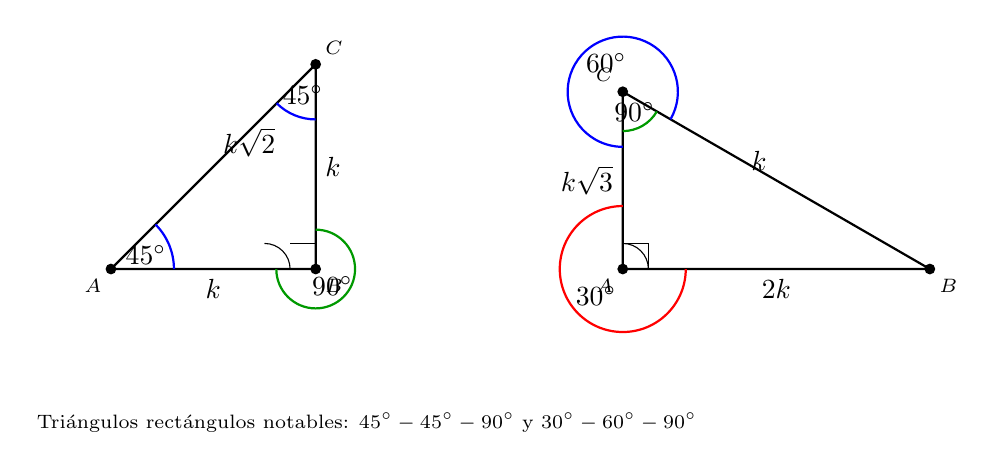
\begin{tikzpicture}[scale=1.3]

  % Triángulo 45°-45°-90° (izquierda)
  \coordinate (A1) at (0,0);
  \coordinate (B1) at (2,0);
  \coordinate (C1) at (2,2);

  \draw[thick] (A1) -- (B1) -- (C1) -- cycle;

  % Ángulo recto
  \draw (1.75,0) arc (0:90:0.25);
  \draw (1.75,0.25) -- (2,0.25) -- (2,0);

  % Ángulos 45°
  \pic["$45^\circ$", draw=blue, thick, angle radius=0.8cm] {angle=B1--A1--C1};
  \pic["$45^\circ$", draw=blue, thick, angle radius=0.7cm] {angle=A1--C1--B1};
  \pic["$90^\circ$", draw=green!60!black, thick, angle radius=0.5cm] {angle=A1--B1--C1};

  % Lados
  \node[below] at (1,0) {$k$};
  \node[right] at (2,1) {$k$};
  \node[above right] at (1,1) {$k\sqrt{2}$};

  % Vértices
  \fill (A1) circle (1.5pt) node[below left] {\scriptsize $A$};
  \fill (B1) circle (1.5pt) node[below right] {\scriptsize $B$};
  \fill (C1) circle (1.5pt) node[above right] {\scriptsize $C$};

  % Triángulo 30°-60°-90° (derecha)
  \begin{scope}[shift={(5,0)}]
    \coordinate (A2) at (0,0);
    \coordinate (B2) at (3,0);
    \coordinate (C2) at (0,1.732);

    \draw[thick] (A2) -- (B2) -- (C2) -- cycle;

    % Ángulo recto
    \draw (0.25,0) arc (0:90:0.25);
    \draw (0,0.25) -- (0.25,0.25) -- (0.25,0);

    % Ángulos
    \pic["$30^\circ$", draw=red, thick, angle radius=0.8cm] {angle=C2--A2--B2};
    \pic["$60^\circ$", draw=blue, thick, angle radius=0.7cm] {angle=B2--C2--A2};
    \pic["$90^\circ$", draw=green!60!black, thick, angle radius=0.5cm] {angle=A2--C2--B2};

    % Lados
    \node[below] at (1.5,0) {$2k$};
    \node[left] at (0,0.866) {$k\sqrt{3}$};
    \node[above left] at (1.5,0.866) {$k$};

    % Vértices
    \fill (A2) circle (1.5pt) node[below left] {\scriptsize $A$};
    \fill (B2) circle (1.5pt) node[below right] {\scriptsize $B$};
    \fill (C2) circle (1.5pt) node[above left] {\scriptsize $C$};
  \end{scope}

  % Título
  \node[font=\scriptsize] at (2.5,-1.5) {Triángulos rectángulos notables: $45^\circ-45^\circ-90^\circ$ y $30^\circ-60^\circ-90^\circ$};

\end{tikzpicture}

\end{document}
